See Fig. \ref{fig:3.8.5_qtwelve}.	Rain velocity 
\begin{align}
\vec{C} -\vec{A} = \myvec{0\\-35}
\end{align}
Woman speed
\begin{align}
\vec{C} -\vec{B} = \myvec{-12\\0}
\end{align}
Relative velocity of rain with respect to the woman is
\begin{align}
 \myvec{0\\-35} - \myvec{-12\\0} = \myvec{12\\-35}
\end{align}
%
Thus, the angle in which the umbrella should be held is
\begin{align}
180\degree - \tan ^{-1}\frac{12}{35}
\end{align}
%
The following python code plots  Fig. \ref{fig:3.8.5_qtwelve}.
	\begin{lstlisting}
	./solutions/5/codes/lines/q12.py
	\end{lstlisting}
\begin{figure}[!ht]
	\centering
	\includegraphics[width=\columnwidth]{./solutions/5/figs/lines/q12.eps}
	\caption{}
	\label{fig:3.8.5_qtwelve}	
	\end{figure}
	


